
%% 
%% Copyright 2007, 2008, 2009 Elsevier Ltd
%% 
%% This file is part of the 'Elsarticle Bundle'.
%% ---------------------------------------------
%% 
%% It may be distributed under the conditions of the LaTeX Project Public
%% License, either version 1.2 of this license or (at your option) any
%% later version.  The latest version of this license is in
%%    http://www.latex-project.org/lppl.txt
%% and version 1.2 or later is part of all distributions of LaTeX
%% version 1999/12/01 or later.
%% 
%% The list of all files belonging to the 'Elsarticle Bundle' is
%% given in the file `manifest.txt'.
%% 
%% Template article for Elsevier's document class `elsarticle'
%% with harvard style bibliographic references
%% SP 2008/03/01

\documentclass[preprint,9pt]{elsarticle}

%% Use the option review to obtain double line spacing
%% \documentclass[authoryear,preprint,review,12pt]{elsarticle}

%% Use the options 1p,twocolumn; 3p; 3p,twocolumn; 5p; or 5p,twocolumn
%% for a journal layout:
%% \documentclass[final,1p,times,authoryear]{elsarticle}
%% \documentclass[final,1p,times,twocolumn,authoryear]{elsarticle}
%% \documentclass[final,3p,times,authoryear]{elsarticle}
%% \documentclass[final,3p,times,twocolumn,authoryear]{elsarticle}
%% \documentclass[final,5p,times,authoryear]{elsarticle}
%% \documentclass[final,5p,times,twocolumn,authoryear]{elsarticle}

%% For including figures, graphicx.sty has been loaded in
%% elsarticle.cls. If you prefer to use the old commands
%% please give \usepackage{epsfig}

%% The amssymb package provides various useful mathematical symbols
\usepackage{amsmath,amssymb,bm}
%\usepackage[dvips,colorlinks=true,citecolor=green]{hyperref}
\usepackage[colorlinks=true,citecolor=green]{hyperref}
%% my added packages
\usepackage{verbatim}
\usepackage{caption}
\usepackage{subcaption}
\usepackage{booktabs} % for nice tables
\usepackage{csvsimple} % for csv read
\usepackage{graphicx}
%\usepackage[outdir=//odroid-sensors/sensors/aidd/reports/journal_papers/MSSP_Paper/Figures/]{epstopdf}
%\usepackage{breqn}
\usepackage{multirow}
% matrix command 
\newcommand{\matr}[1]{\mathbf{#1}} % bold upright (Elsevier, Springer)
% vector command 
\newcommand{\vect}[1]{\mathbf{#1}} % bold upright (Elsevier, Springer)
\newcommand{\ud}{\mathrm{d}}
\renewcommand{\vec}[1]{\mathbf{#1}}
\newcommand{\veca}[2]{\mathbf{#1}{#2}}
\renewcommand{\bm}[1]{\mathbf{#1}}
\newcommand{\bs}[1]{\boldsymbol{#1}}
\graphicspath{{Figures/}{//odroid-sensors/sensors/aidd/reports/journal_papers/MSSP_Paper/Figures/}}
%\graphicspath{ {Graphics/Figures/} }
%% The amsthm package provides extended theorem environments
%% \usepackage{amsthm}
%% The lineno packages adds line numbers. Start line numbering with
%% \begin{linenumbers}, end it with \end{linenumbers}. Or switch it on
%% for the whole article with \linenumbers.
%% \usepackage{lineno}
\journal{Mechanical Systems and Signal Processing}

\begin{document}
	\begin{frontmatter}
		\addcontentsline{toc}{section}{References}
		%% Title, authors and addresses
		%% use the tnoteref command within \title for footnotes;
		%% use the tnotetext command for theassociated footnote;
		%% use the fnref command within \author or \address for footnotes;
		%% use the fntext command for theassociated footnote;
		%% use the corref command within \author for corresponding author footnotes;
		%% use the cortext command for theassociated footnote;
		%% use the ead command for the email address,
		%% and the form \ead[url] for the home page:
		%% \title{Title\tnoteref{label1}}
		%% \tnotetext[label1]{}
		%% \author{Name\corref{cor1}\fnref{label2}}
		%% \ead{email address}
		%% \ead[url]{home page}
		%% \fntext[label2]{}
		%% \cortext[cor1]{}
		%% \address{Address\fnref{label3}}
		%% \fntext[label3]{}
		
		\title{Full Wavefield Processing by Using FCN for Delamination Detection}
		
		%% use optional labels to link authors explicitly to addresses:
		%% \author[label1,label2]{}
		\address[IFFM]{Institute of Fluid Flow Machinery, Polish Academy of Sciences, Poland}
		
		\author{Abdalraheem A. Ijjeh\fnref{IFFM}}
		\author{Saeed Ullah \fnref{IFFM}}
		\author{Pawel Kudela\corref{cor1}\fnref{IFFM}}
		\ead{pk@imp.gda.pl}
		%\ead{pfiborek@imp.gda.pl}
		%\author{Tomasz Wandowski \fnref{IFFM}}	
		
		\cortext[cor1]{Corresponding author}
		
		\begin{abstract}
		
		\end{abstract}
		
		\begin{keyword}
			%% keywords here, in the form: keyword \sep keyword
			Lamb waves \sep structural heath monitoring \sep damage detection \sep deep learning \sep Convolutional neural networks CNN. \sep fully convolutional neural network FCN
			%% PACS codes here, in the form: \PACS code \sep code
			
			%% MSC codes here, in the form: \MSC code \sep code
			%% or \MSC[2008] code \sep code (2000 is the default)
			
		\end{keyword}
		
	\end{frontmatter}
	%% main text

%%%%%%%%%%%%%%%%%%%%%%%%%%%%%%%%%%%%%%%%%%%%%%%%%%%%%
\section{Introduction}
%%%%%%%%%%%%%%%%%%%%%%%%%%%%%%%%%%%%%%%%%%%%%%%%%%
Composite materials have a wide range of applications in various industries, due to their characteristics such as high strength, low density, resistance to fatigue, and corrosion.  
However, damage can occur in composites materials due to impacts resulting from the lack of reinforcement in the out-of-plane direction~\cite{Francesconi2019}.
In particular, laminated composite materials are more sensitive to delamination damage due to weak transverse tensile and interlaminar shear strengths.
Delamination can alter the compression strength of composite laminate, and gradually affect the composite to encounter failure by buckling. 
Delaminations can seriously decrease the performance of composites structures, accordingly, delamination detection in its early stages can significantly help to avoid catastrophic structural collapses.
	
One of the conventional techniques for damage identification for non-destru\-ctive testing (NDT) involves arrays of transducers that can be mounted or embedded in the structures for registering the response of the guided wave propagation.
However, damage identification regarding structures with curved and deformable geometry can be inaccurate when using an array of transducers.
Also, damage influence maps resulted from processing of signals registered by the array of transducers have low resolution, due to the small number of sensing points. 
Accordingly, this issue of low resolution damage influence map can be solved by utilising a Scanning Laser Doppler Vibrometry (SLDV), which is a non-contact technique dedicated to full wavefield measurements of vibration and guided wave propagation.
The measurements are conducted on a dense mesh of measurement points spanned over the area of the investigated structure.
Consequently, SLDV produces a full wavefield of measurements with high resolution of damage influence maps which can significantly improve the process of damage detection and localization~\cite{Michaels2007,Park2014,Tian2015a,Kudela2015}.
Full wavefield processing techniques even allow for damage size estimation~\cite{Girolamo2018a,Kudela2018} which is difficult to perform in case of transducer arrays especially for composite structures.
Therefore, the latter methods are evaluated mostly for damage detection and localisation in metallic structures~\cite{Michaels2008,Huang2018a,Wang2020}.

Certain algorithms such as the time reversal algorithm can benefit from combining piezoceramic transducers (as actuators) with SLDV for sensing~\cite{Girolamo2018a, Miniaci2019}.
    
Conventional damage detection and localization methods focus on patterns extraction from registered measurements and accordingly make decisions based on these patterns ~\cite{Gul2009}. 
Moreover, conventional methods for pattern recognition requires feature selection and classification (handcrafted features). 
These conventional methods can perform efficient damage detection, however, these methods depend on selected features from their scope of measurement.
Accordingly, introducing new patterns will cause them to fail in detecting the damage.
Moreover, these methods could fail in detecting damage when dealing with big data requiring a complex computation of damage features~\cite{Gulgec2019}.
Perhaps the most challenging part for damage detection is determining the unknown relationship between registered measurements and damage patterns~\cite{Gulgec2019}. 
    
The accelerated progress in the field of artificial intelligence (AI) technologies in recent years, and mainly in deep learning, revealed new dimensions for solving problems and offered the opportunity for being implemented and integrated with the NDT and further with structural health monitoring (SHM) approaches.
Therefore, issues regarding data preprocessing and feature extraction can be handled when applying deep learning techniques. 
Nowadays, end-to-end approaches are presented, in which the whole unprocessed data are fed in the model, hence, it will learn by itself to recognise the patterns and detect the damage.
    
%%%%%%%%%%%%%%%%%%%%%%%%%%%%%%%%%%%%%%%%%%%%%%%%%%%%%
In the following, methods for damage size estimation based on machine learning and deep learning techniques are presented which are targeted in the field of SHM/NDT.
  	
%%%%%%%%%%%%%%%%%%%%%%%%%%%%%%%%%%%%%%%%%%%%%%%%%%%%%
One of the earliest work for delamination location and size assessment in composite structures using deep learning techniques was performed by Islam et al.~\cite{islam1994damage}. 
They have trained a neural network model with frequencies for the first five modes obtained from modal analysis data. 
The data was acquired by piezoceramic sensors in both damaged and undamaged composite beams.
 %%%%%%%%%%%%%%%%%%%%%%%%%%%%%%%%%%%%%%%%%%%%%%%%%%%%%
 Okafor et al~\cite{okafor1996delamination} applied a feed-forward backpropagation neural network to assess the delamination size in a smart composite beam. 
 For training the neural network model, authors used delamination sizes and corresponding the first four modal frequencies. 
 The trained model was tested with new cases of delamination using the first four normalized frequencies of test cases as an input to the network. 
 Their model predicted the delamination size between 0.22~cm and 0.82~cm successfully.
 %%%%%%%%%%%%%%%%%%%%%%%%%%%%%%%%%%%%%%%%%%%%%%%%%%%%%
 Moreover, Chakraborty et al.~\cite{chakraborty2005artificial} proposed a neural network model for detecting delamination shape, size and location in a fibre reinforced plastic composite laminate.
 Authors used natural frequencies as inputs and the corresponding size, shape and location of delamination as outputs of the model. 
 %%%%%%%%%%%%%%%%%%%%%%%%%%%%%%%%%%%%%%%%%%%%%%%%%%%%%
 Authors in ~\cite{roseiro2005neural}  proposed a damage detection method in laminated composite plates to locate and quantify damage through utilising the electrical potential of piezoelectric sensors and artificial neural networks. 
 The model was trained using the Levenberg-Marquardt algorithm. High accuracy of damage location was achieved.
 But tests were performed only based on the numerical model.  
 %%%%%%%%%%%%%%%%%%%%%%%%%%%%%%%%%%%%%%%%%%%%%%%%%%%%%

 Sammons et al.~\cite{sammons2016segmenting}, utilised X-ray computed tomography for estimating the delaminations in a CFRP. 
 For this purpose, they utilised the convolutional neural network (CNN) for performing image segmentation of the defected input images to estimate the delaminations. 
 Their ConvNet was capable of identifying and quantifying small delaminations. 
 Unfortunately, the ConveNet could not recognise delaminations with large sizes.
 %%%%%%%%%%%%%%%%%%%%%%%%%%%%%%%%%%%%%%%%%%%%%%%%%%%%%
 
 Further, De Fenza et al.~\cite{de2015application} proposed a method for damage detection for aluminium and composite materials plates using Lamb waves by a neural network model for automatic feature extraction and probability ellipse based method. 
 The neural network model and probability ellipse were applied on the damage index (DI) computed by comparing the differences in the measured  Lamb waves prior and post the damage occurrence. 
  %%%%%%%%%%%%%%%%%%%%%%%%%%%%%%%%%%%%%%%%%%%%%%%%%%%%%
 Ewald et al.~\cite{ewald2019deepshm} proposed a deep learning technique for SHM on guided Lamb waves "DeepSHM". 
 They pre-processed the sensor signal response through applying wavelet transform to obtain the wavelet coefficient matrix (WCM), which is fed into the CNN for training to acquire the neural weights. 
 They achieved different classification accuracies ranging from \(\%17\) to \(\%99.9\).
  %%%%%%%%%%%%%%%%%%%%%%%%%%%%%%%%%%%%%%%%%%%%%%%%%%%%
  %%%%%%%%%%%%%%%%%%%%%%%%%%%%%%%%%%%%%%%%%%%%%%%%%%%%%
 Authors in~\cite{Melville2018} proposed a technique for damage detection in thin metal plates (aluminum and steel), using full wavefield data acquired by SLDV. 
 Using this data to train a deep neural network of 4 hidden layers including 2 convolutional layers for features extraction and 2 fully connected layers. 
 Their results show good results when compared with traditional support vector machine (SVM) methods.
 %%%%%%%%%%%%%%%%%%%%%%%%%%%%%%%%%%%%%%%%%%%%%%%%%%%%% 
%%%%%%%%%%%%%%%%%%%%%%%%%%%%%%%%%%%%%%%%%%%%%%%%%%%%%
Furthermore, Esfandabadi et al.~\cite{esfandabadideep} applied 20 layers based very-deep super-resolution (VDSR) architecture, (VDSR is a variant of CNN) on a guided ultrasonic wavefield for enhancing quality of image resolution and quality of the acquired wavefield. 
VDSR was applied in conjunction with compressive sensing theory with the aim of reducing the acquisition time of the ultrasonic wavefield.
The model was trained on \(652\) wavefield images (\(326\) with defect) and (\(326\) without defects) generated by piezoelectric transducers and acquired by SLDV. 
Authors have used various aluminium and CFRP plates to prepare the dataset.
It was concluded that high-resolution images can be obtained, even when only the 10\% of the original scan points were retained.
%%%%%%%%%%%%%%%%%%%%%%%%%%%%%%%%%%%%%%%%%%%%%%%%%%%%%

Motivated by high potentials of deep learning techniques, in this work, we are exploring the feasibility of applying such techniques for detecting delaminations in CFRP plates. 
One of the key points of our work is the computation of a large dataset of full wavefield of propagating guided waves by using the parallel version of the time domain spectral element method~\cite{Kudela2020}. 
Numerically generated data resembles measurements acquired by SLDV. 
	
For our knowledge, it is the first time, a large full wavefield dataset of propagating guided waves will be fed as an input to deep neural networks with the aim of delamination size estimation.

In this work, we are presenting a pixel-wise segmentation model which is capable of detecting and localising the delamination, through segmentation of the input image into damaged and undamaged parts.
Moreover, the pixel-wise segmentation model enables the precise shape and size estimation of defects.
The capabilities and potentials of the proposed method are compared to the conventional wavefield signal processing method i.e. adaptive wavenumber filtering~\cite{Kudela2015,Radzienski2019}.
The quantitative comparison was performed by using intersection over the union of detected delamination area with respect to the ground truth. 

%%%%%%%%%%%%%%%%%%%%%%%%%%%%%%%%%%%%%%%%%%%%%%%%%%%%%
	\section{Methodology}
	%%%%%%%%%%%%%%%%%%%%%%%%%%%%%%%%%%%%%%%%%%%%%%%%%%%%%
	%%%%%%%%%%%%%%%%%%%%%%%%%%%%%%%%%%%%%%%%%%%%%%%%%%%%%
	\subsection{Dataset}
	%%%%%%%%%%%%%%%%%%%%%%%%%%%%%%%%%%%%%%%%%%%%%%%%%%%%%
	In this work, we have generated a large dataset of 475 cases of a full wavefield of propagating Lamb waves in a plate made of carbon fibre-reinforced plastic (CFRP).
	The time-domain spectral element method was used for simulation of Lamb wave interaction with delamination~\cite{Kudela2020}.
	For each case, single delamination was modelled by using the method of splitting nodes between appropriate spectral elements. 
	It was assumed that the composite laminate is made of eight layers of a total thickness of 3.9 mm.
	The delamination was modelled between the third and fourth layer (see Fig.~\ref{fig:plate_setup} for details).
	It should be noted that the figure shows an exaggerated cross-section through the delamination. 
	Zero-volume delamination was assumed in the model. 
	For each case delamination location was selected randomly so that interaction of guided waves excited at the plate centre with delamination is different for each case.
	It includes cases when delamination is located at the edge of the plate which is the most difficult to identify by signal processing methods.
	Additionally, the size of the delamination was randomly simulated by selecting the ellipse minor and major axis from the interval 10--40 mm.
	Also, the angle between the delamination major axis and the horizontal axis was randomly selected.
	\begin{figure}
		\centering
		\includegraphics[scale=0.8]{plate_delam_arrangement_MSSP.png}
		\caption{Setup for computing Lamb wave interactions with delamination.}
		\label{fig:plate_setup}
	\end{figure}

	The output from the top and bottom surface of the plate in the form of particle velocities at the nodes of spectral elements were projected on the uniform grid of 500\(\times\)500 points by using shape functions of elements (see Parallel spectral element method for guided wave based structural health monitoring paper for detail).
	It essentially resembles measurements acquired by SLDV in the transverse direction (perpendicular to the plate surface).

	%%%%%%%%%%%%%%%%%%%%%%%%%%%%%%%%%%%%%%%%%%%%%%%%%%%%
\subsection{Signal processing strategy}
%%%%%%%%%%%%%%%%%%%%%%%%%%%%%%%%%%%%%%%%%%%%%%%%%%%%
Two signal processing strategies are applied: newly proposed image processing based on the FCN and conventional one which is the adaptive wavenumber filtering.
The former one is represented by the left branch on the scheme shown in~Fig.~\ref{fig:sig_proc_strategy} whereas the latter one is represented by the right branch.
The starting point for both approaches is the dataset consisted of frames of propagating guided waves.
However, the FCN takes as an input the RMS which combines all frames into one image. 
It essentially represents the spatial energy distribution of propagating waves.
In the adaptive wavenumber filtering method, all frames are utilised (right branch of Fig.~\ref{fig:sig_proc_strategy}).
The RMS is applied later on to output final damage map in the form of an image.

It should be noted that we tested two types of activation functions as a last layer of the FCN: softmax and sigmoid.
The former one gives the binary output which segments pixels in two categories: damaged and undamaged.
On the other hand, the threshold needs to be applied when the sigmoid activation function is used.
Also, damage maps resulted from the adaptive wavenumber filtering must be thresholded so that the area and shape of delamination can be estimated.

Finally, intersection over union (IoU) is applied as a measure of delamination size, shape and location so that all presented approaches can be compared quantitatively. 
	\begin{figure}
		\centering
		\includegraphics[scale=0.8]{FCN_adaptive_filtering_diagram_MSSP.png}
		\caption{Diagram of signal processing strategy by the proposed Fully Convolutional Network (left branch) in comparison to signal processing utilising adaptive wavenumber filtering method (right branch). }
		\label{fig:sig_proc_strategy}
	\end{figure}
The particular blocks presented in the Fig.~\ref{fig:sig_proc_strategy} will be explained in more details in the next sections.
	
%%%%%%%%%%%%%%%%%%%%%%%%%%%%%%%%%%%%%%%%%%%%%%%%%%%%	
\subsection{Adaptive wavenumber filtering}
%%%%%%%%%%%%%%%%%%%%%%%%%%%%%%%%%%%%%%%%%%%%%%%%%%%%
Adaptive wavenumber filtering is a well-established method for processing of images of propagating elastic waves.
The method has proved to be useful for crack size estimation~\cite{Kudela2015}, impact induced damage assessment~\cite{Kudela2018},  delamination and disbonding detection and localisation~\cite{Radzienski2019}.  
It is used here as a reference point for comparison purposes against proposed strategies based on FCN.

The method involves steps such as 2D Fourier Transform, wavenumber filtering, inverse Fourier Transform and RMS.
It can be used as an automated tool for producing damage maps which are easy in interpretation.
However, it still requires setting a threshold for the filter mask and quantisation threshold useful for damage size estimation.
These thresholds can be estimated empirically and even certain rigid range of thresholds will lead to satisfactory results.
Nevertheless, it is not a fully automatic process.
FCN based approach seems to have an advantage in this regard.

	%%%%%%%%%%%%%%%%%%%%%%%%%%%%%%%%%%%%%%%%%%%%%%%%%%%%%
	\subsection{Fully Convolutional Network approach}
	%%%%%%%%%%%%%%%%%%%%%%%%%%%%%%%%%%%%%%%%%%%%%%%%%%%%%
	In this section, a deep learning approach for delamination detection in composite materials is presented. 
	%%%%%%%%%%%%%%%%%%%%%%%%%%%%%%%%%%%%%%%%%%%%%%%%%%%%%
	\subsubsection{Data preprocessing}
	%%%%%%%%%%%%%%%%%%%%%%%%%%%%%%%%%%%%%%%%%%%%%%%%%%%%%
	It should be noted that the output from the wave propagation model is in the form of 3D matrix which contains amplitudes of propagating waves at location \((x, y)\) and time \(t\). We can look at it as a set of frames of propagating waves at discrete time moments \(t_k\).

	The data preprocessing as it is indicated in Fig.~\ref{fig:sig_proc_strategy} include a step of computation of root mean square value:
	\begin{equation}
		\hat{s}(x,y) = \sqrt{\frac{1}{N}\sum_{k=1}^{N} s(x,y,t_k)^2}
		\label{eq:rms}
	\end{equation}
	where the number of sampling points \(N\) was 512.
	In this way, the dataset was collapsed to 475 2D matrices in which amplitudes are stored as double-precision values.
	The next step was the conversion of these matrices to greyscale images (colour image quantisation).
	Colour scale values of obtained images vary between (\(0 - 255\)) hence normalization
	to a range of (\(0-1\)) was applied to enhance the optimizer function during the learning process. 
	
	Furthermore, data augmentation was achieved by flipping images horizontally, vertically and diagonally. 
	It increased the dataset size four times -- \(1900\) images were produced.
	
	Such data augmentation can enhance the learning process by enabling the model to learn and recognize new complex patterns.
	
<<<<<<< HEAD
	Initially, we split the dataset into three portions: \(80\%\) for the training set, \(20\%\) for testing set and \(20\%\) of the training set as separated to the validation set.
=======
	The data set was split into two portions:  \(80\%\) for the training set and \(20\%\) for the testing set.
	Additionally, the validation set was created as a \(20\%\) of the training set.
>>>>>>> 3b1c1b0e9161c1ff09015d843b5d94014da98734
	%%%%%%%%%%%%%%%%%%%%%%%%%%%%%%%%%%%%%%%%%%%%%%%%%%%%%
	%%%%%%%%%%%%%%%%%%%%%%%%%%%%%%%%%%%%%%%%%%%%%%%%%%%%%
\subsection{Methodology}
%%%%%%%%%%%%%%%%%%%%%%%%%%%%%%%%%%%%%%%%%%%%%%%%%%%%%
The main purpose of utilizing deep learning methods is to perform the feature extraction process automatically through feeding the models the full wavefield images.
Therefore, the models will learn by themself to recognise different and complex patterns, consequently identify the delamination. 
In this work, we have done a comparative study among several deep learning models based on fully convolutional networks (FCN)~\cite{shelhamer2017fully} that aim to perform pixel-wise segmentation by classifying every pixel of the input image as damaged or not. 

FCN is built by stacking convolutional layers in an encoder-decoder scheme, therefore, dense layers are not included in FCN models. 
The idea behind the encoder is to extract condensed feature maps of the input image through downsampling that is performed by applying several convolutions with strides.
The decoder part is responsible for upsampling the condensed features maps to the same size of the original input image by using techniques like transposed convolution with strides and upsampling with interpolation.

%In order to reduce overfitting in the models, some techniques were applied such as adding dropouts to layers and batch normalization in addition to early mentioned Kfold CV method.

For all implemented models in this comparative study, we have used a softmax activation function at the output layer.
The softmax function computes the probability of the damaged and undamaged occurrence for every single pixel.
Consequently, the sum of the two probabilities must be one. 
Eq.~(\ref{softmax}) illustrates the softmax, where \(P(x)_{i}\) is the probability of each target class \(x_{j}\) over all possible target classes \(x_{j}\), C in our case are two classes  (damaged and undamaged).
To predict the label of the detected output (\(y_{pred}\)) that represent the damaged and undamaged probabilities, an \(\argmax\) function is applied to select the maximum probability between both of them.
	\begin{equation}
		P(x)_{i} = \frac{e^{x_{i}}}{\sum_{j}^{C} e^{x_{j}}}
		\label{softmax}
	\end{equation} 
	\begin{equation}
		y_{pred} = \argmax_{i}\left( P(x)_{i} \right)
		\label{argmax}
	\end{equation}
In deep learning models, choosing a suitable loss function is an important task because it measures how good the model is performing.
In our implemented models, we have applied the categorical cross-entropy loss function, which is also called \enquote{softmax loss function}.
Eq.~(\ref{CCE}) illustrates the CCE, where \( P(x)_{i}\) is the softmax value of the target class. 
	\begin{equation}
	CCE = -\log\left( P(x)_{i} \right)
	\label{CCE}
	\end{equation}

Additionally, it is also important to select a proper accuracy metric of the model, therefore, we have applied intersection over union (IoU) as our accuracy metric. 
IoU is estimated by determining the intersection area between the ground truth and the predicted output.  
The IoU metric is defined as:
\begin{equation}
IoU = \frac{Intersection}{Union} = \frac{\hat{Y} \cap Y}{\hat{Y} \cup Y} 
\label{IoU}
\end{equation}
The IoU can be calculated by multiplying the predicted output with its ground truth value to find the intersection, and it divided over the union which can be calculated by counting all pixel values greater than zero of the predicted output and its ground truth.
%As we mentioned earlier the ground truth values are either \((0\) or \(1)\) thus only the predicted values larger than \(0\) multiplied by their ground truth label \(1\) will be counted, the rest values will equal to \(0\). 
%The union can be calculated by summing all values in both the predicted and the ground truth  vectors, then we subtract the intersection from their sum.
In order to increase the IoU and to reduce the loss during the training, we have applied Adam optimizer which is considered as a combination of RMSprop and stochastic gradient descent (SGD)~\cite{Kingma2015}. 
The purpose of the optimizer is to change the learnable parameters such as the weights of the filters and biases in a way the loss is reduced and the accuracy metric is increased.

In the next subsections, we present several FCN models for pixel-wise semantic segmentation to detect and localise delaminations.

	\subsubsection{U-Net based model}
%%%%%%%%%%%%%%%%%%%%%%%%%%%%%%%%%%%%%%%%%%%%%%%%%%%%
U-Net is a well-known architecture based on encoder-decoder scheme was introduced by Ronneberger et al.~\cite{Ronneberger2015} for biomedical image segmentation. 
The principle function of the encoder is to capture the context of an input image, while the decoder is responsible for enabling a precise localisation. 
%U-net is composed of three parts: The downsampling section, The bottleneck, and the upsampling section. 
%%%%%%%%%%%%%%%%%%%%%%%%%%%%%%%%%%%%%%%%%%%%%%%%%%%%%%%%%%%%%%%%%%%%%%%%%%%%%%%%%%%%%%%%
The encoder part holds several downsampling blocks. 
Each block takes an input applies two convolutional layers followed by a (\(2\times2\)) max pooling with a (\(2\times2\)) strides that picks the maximum value in a local pool filter in one feature map (or \(n\)-feature maps), resulting in a reduction in the dimension of feature maps~\cite{Lecun2015}, consequently, reducing computation complexity.
Each convolutional layer performs (\(3\times3\)) convolution operations, followed by Relu activation function.
Furthermore, to enhance the model training performance we applied batch normalization (BN)~\cite{Ioffe2015} after each convolutional layer.
Moreover, the number of convolutional filters is doubled after each downsampling block therefore the model can learn complex patterns effectively. 
%%%%%%%%%%%%%%%%%%%%%%%%%%%%%%%%%%%%%%%%%%%%%%%%%%%%%%%%%%%%%%%%%%%%%%%%%%%%%%%%%%%%%%%%
The bottleneck layer meddles between the encoder and the decoder as a joining point is the deepest layer in the model.
The bottleneck contains two convolutional layers, with 256 filters which helps the model to learn and recognize the complex patterns.
%It composed of two (\(3\times3\)) convolution layers followed by (\(2\times2\)) up convolution layer (Transpose convolution).
%%%%%%%%%%%%%%%%%%%%%%%%%%%%%%%%%%%%%%%%%%%%%%%%%%%%%%%%%%%%%%%%%%%%%%%%%%%%%%%%%%%%%%%%
The decoder consists of several upsampling blocks. 
Each upsampling block passes the input into two convolution layers as in the downsampling block followed by a transmission up layer consists of a transposed convolutional layer (upsampling). 
The purpose of upsampling is to retrieve the dimensions and increase the resolution.
Transposed convolutional layer differs from the regular upsampling function, by introducing learnable parameters regarding the transposed convolution filters that enhance the learning process of the model. 
Moreover, after each upsampling operation, the number of feature maps used by convolutional layer reduced by half to keep the model symmetrical. 
Further, skip connections were added by appending feature maps of the downsampling block with the corresponding upsampling block to retrieve lost spatial information during the downsampling due to the reduction of the input resolution.
Therefore, the model ensures that the feature maps which were learned during the downsampling will be utilized in the reconstruction. 
%%%%%%%%%%%%%%%%%%%%%%%%%%%%%%%%%%%%%%%%%%%%%%%%%%%%%%%%%%%%%%%%%%%%%%%%%%%%%%%%%%%%%%%%
\begin{figure} [h!]
	\begin{center}
		\includegraphics[scale= 0.8]{Unet_model.png}
	\end{center}
	\caption{U-Net architecture.} 
	\label{fig:Unet}
\end{figure}
Fig.~\ref{fig:Unet}  illustrates the network architecture. 
The encoder is on the left side in which the downsampling is performed and the decoder is on the right side where the upsampling is performed in addition to the bottleneck where is join both sides.
%%%%%%%%%%%%%%%%%%%%%%%%%%%%%%%%%%%%%%%%%%%%%%%%%%%%%
\subsubsection{VGG16 encoder-decoder}
%%%%%%%%%%%%%%%%%%%%%%%%%%%%%%%%%%%%%%%%%%%%%%%%%%%%%
In this model, we address the use of VGG16 architecture  ~\cite{simonyan2014very} as a backbone encoder to the U-Net architecture.
VGG16 is composed of 13 convolutional layers, pooling layers and dense layers, and it is used for classification purposes. 
We applied VGG16 encoder-decoder for pixel-wise image segmentation.
Figure~\ref{vgg16} presents the architecture of VGG16 encoder-decoder model. 
The model consists of two parts: downsampling and upsampling.
The downsampling path consists of \(5\) convolutional blocks,  with a total \(13\) convolutional layers  with \enquote{same} padding with a kernel size (\(3\times3\))and 32 filters for each layer, followed by BN and activation function Relu.
Each convolutional layer is responsible for extracting high level features from the input image such as edges.
A Maxpool operation with pool size of (\(2\times2\))  and (\(2\times2\)) strides followed by dropout is performed after each convolutional block. 
The upsampling path is introduced to recover spatial resolution, it also has \(5\) convolutional blocks with a total \(13\) convolutional layers  with same padding and kernel size (\(3\times3\))and 32 filters for each layer, followed by BN and activation function Relu.
For upsampling, bilinear interpolation with (\(2\times2\)) kernel size is applied.
Skip connections were added between downsampling blocks and the corresponding upsampling blocks in order to enhance recovering fine-grained details by enabling feature re-usability from earlier layers.
\begin{figure} [h!]
	\begin{center}
		\includegraphics[scale=1]{VGG16_encoder_decoder.png}
	\end{center}
	\caption{VGG16 encoder decoder architecture.} 
	\label{vgg16}
\end{figure}
%%%%%%%%%%%%%%%%%%%%%%%%%%%%%%%%%%%%%%%%%%%%%%%%%%%%
\subsubsection{FCN-DenseNet model}
%%%%%%%%%%%%%%%%%%%%%%%%%%%%%%%%%%%%%%%%%%%%%%%%%%%%%	
FCN-DenseNet which was introduced in~\cite{Jegou} was applied in our previous work~\cite{Ijjeh2021} for image segmentation.
The results were promising since it outperformed the conventional damage detection technique i.e (adaptive wavenumber filtering method). 
FCN-DenseNet has a U-shape of the encoder-decoder scheme with skip connections between the downsampling and the upsampling paths to increase the resolution to the final feature map.
The main component in FCN-DenseNet is the dense block.
The dense block is constructed from \(n\) varying number of layers, each layer consists of a series of operations as shown in Table~\ref{layers}.
The purpose of the dense block is to concatenate the input (\(x\)) (feature maps) of a layer with its output (feature maps) to emphasize spatial details information.
In this work, we have updated the FCN-DenseNet model by increasing the number of dense blocks and the learnable parameters (filters).
The architecture of the dense block is presented in Fig.~\ref{dense_block}. 
\begin{figure} [h!]
	\begin{center}
		\includegraphics[scale=1.0,angle=-90]{figure6.png}
	\end{center}
	\caption{Dense block architecture.} 
	\label{dense_block}
\end{figure}
%%%%%%%%%%%%%%%%%%%%%%%%%%%%%%%%%%%%%%%%%%%%%%%%%%%%%%%%%%%%%%%%%%%%
To reduce the spatial dimensionality of the produced feature maps, a transition down layer was added to perform a (\(1\times 1\)) convolution followed by (\(2\times2\)) Maxpooling operation. 
%%%%%%%%%%%%%%%%%%%%%%%%%%%%%%%%%%%%%%%%%%%%%%%%%%%%%%%%%%%%%%%%%%%%
Consequently, to recover the spatial resolution, a transition-up layer was added. 
It applies a transpose convolution operation to upsample feature maps from the previous layer.
%%%%%%%%%%%%%%%%%%%%%%%%%%%%%%%%%%%%%%%%%%%%%%%%%%%%%%%%%%%%%%%%%%%%
Feature maps emerging from upsampling are concatenated with the ones resulting from the skip connection forming the input to a new dense block.
During the upsampling, the input to the dense block is not concatenated with its output to overcome the overhead of memory shortage since the upsampling path expands the spatial resolution of the feature maps. 
%(hint:- We can refer to previous paper and say that the same architecture was applied here. Than we can skip Fig.~\ref{fcn}).
%\begin{figure} [h!]
%	\begin{center}
%		\includegraphics[scale=1.0]{FCN_dense_net.png}
%	\end{center}
%	\caption{FCN-DenseNet architecture.} 
%	\label{fcn}
%\end{figure}
Table~\ref{layers} presents the architecture of a single layer, the transition down  and transition up layers in details.
%Figure~\ref{fcn} illustrates the FCN-DenseNet architecture for image segmentation used for delamination detection.
%%%%%%%%%%%%%%%%%%%%%%%%%%%%%%%%%%%%%%%%%%%%%%%%%%%%%%%%%%%%%%%%%%%%
\begin{table}[h!]
	\renewcommand{\arraystretch}{1.3}
	\centering
	\scriptsize
	\resizebox{\textwidth}{!}
	{
	\begin{tabular}{ccccc}
		\hline
		Layer &  &  Transition Down &  &  Transition Up \\ 
		\hline
		Batch Normalization &  & Batch Normalization &  &  \(3\times 3\) Transposed Convolution  \\ 
		Relu &  & Relu &  & strides = (\(2\times2\))  \\ 
		(\(3\times3\)) Convolution &  & (\(1\times1\)) Convolution &  &  \\ 
%		&  &   \\ 
		Dropout \(p=0.2\) &  &Dropout \(p=0.2\)  &  &  \\ 
		 &  & (\(2\times2\)) Maxpooling &  &  \\ 
	    \hline
	\end{tabular}
	}
	\caption{Layer, Transition Down and Transition Up layers.} 
	\label{layers}
	
\end{table}\\



	%%%%%%%%%%%%%%%%%%%%%%%%%%%%%%%%%%%%%%%%%%%%%%%%%%%%%
	\section{Results and discussions}
\label{section:results_and_discussions}
%%%%%%%%%%%%%%%%%%%%%%%%%%%%%%%%%%%%%%%%%%%%%%%%%%%%%%%%%%%%%%%%%%%%%%%%%%%%%%%%
In this section, five DL models  of semantic segmentation approach including  Res-UNet, VGG16 encoder-decoder, FCN-DenseNet, PSPNet and GCN were evaluated on exemplary three damage scenarios of an RMS of the full wavefield interpolated at the bottom surface of the plate (numerically generated) in order to identify the delamination.
Additionally, an experimental scenario was also used to evaluate the performance of the models to show the DL capabilities of generalization.
For each model, the mean and the max \(IoU\) are calculated and presented as a metric of comparison.
Moreover, the Accuracy of classification, Precision, Recall, and F1-score depicted in Eqs~(\ref{accuracy}-\ref{f1_score}) respectively, were calculated for each model.
\begin{equation}
	\rm Accuracy\ = \frac{TP+TN}{(Total\ number\ of\ tested\ samples)}
	\label{accuracy}
\end{equation}

\begin{equation}
	\rm Pricision\ =\frac{TP}{TP+FP}
	\label{pricisoin}
\end{equation}
\begin{equation}
	\rm Recall\ = \frac{TP}{TP+ FN}
	\label{recall}
\end{equation}
\begin{equation}
	\rm F1-Score =\frac{2 \times (Pricision\times Recall)}{(Pricision + Recall)} 
	\label{f1_score}
\end{equation}
where the Positive/Negative refers to the predicted output as (damage or non-damage) respectively, True Positive (TP) and True Negative (TN)  represent the correct classification, and the False Positive (FP) and False Negative (FN) represent the incorrect classification.

In our work, all semantic segmentation models were implemented and trained with Keras API~\cite{chollet2015keras} (an open-source platform) running on top of TensorFlow on an NVIDIA Tesla V100 GPU. 
Moreover, for training purposes, we have used K-fold CV technique with \(k=5\). Accordingly, each model has been trained for \(5\) iterations, then the mean accuracy of all folds is calculated. 
Further, for each iteration, the models were trained on the augmented dataset up to \(20\) epochs.
%%%%%%%%%%%%%%%%%%%%%%%%%%%%%%%%%%%%%%%%%%%%%%%%%%%%%%%%%%%%%%%%%%%%%%%%%%%%%%%%

The first exemplary delamination scenario is shown in Fig.~\ref{fig:softmax_448}. 
The delamination is located at the left edge of the plate and its corresponding ground truth image are shown in Fig.~\ref{fig:RMS_flat_shell_Vz_448} and ~\ref{fig:m1_rand_single_delam_448} respectively. 
Figures~\ref{fig:unet_pred_448} -~\ref{fig:gcn_pred_448} show the predicted output of the Res-UNet, VGG16 encoder-decoder, PSPNet, FCN-DenseNet and GCN models, respectively. 
%%%%%%%%%%%%%%%%%%%%%%%%%%%%%%%%%%%%%%%%%%%%%%%%%%%%%%%%%%%%%%%%%%%%%%%%%%%%%%%%
\begin{figure} [!h]
	\centering
	\begin{subfigure}[b]{0.47\textwidth}
		\centering
		\includegraphics[scale=1.0]{RMS_flat_shell_Vz_448_500x500bottom.png}
		\caption{RMS bottom}
		\label{fig:RMS_flat_shell_Vz_448}
	\end{subfigure}
	\hfill
	\begin{subfigure}[b]{0.47\textwidth}
		\centering
		\includegraphics[scale=1.0]{m1_rand_single_delam_448.png}
		\caption{Ground truth}
		\label{fig:m1_rand_single_delam_448}
	\end{subfigure}
	\begin{subfigure}[b]{0.47\textwidth}
		\centering
		\includegraphics[scale=1.0]{residual_unet_num_269.png}
		\caption{Res-UNet}
		\label{fig:unet_pred_448}
	\end{subfigure}
	\hfill
	\begin{subfigure}[b]{0.47\textwidth}
		\centering
		\includegraphics[scale=1.0]{VGG16_ecoder_decoder_num_269.png}
		\caption{VGG16 encoder-decoder}
		\label{fig:vgg16_pred_448}
	\end{subfigure}
	\hfill
	\begin{subfigure}[b]{0.47\textwidth}
		\centering
		\includegraphics[scale=1.0]{PSPNet_num_269.png}
		\caption{PSPNet}
		\label{fig:pspnet_pred_448}
	\end{subfigure}
	\hfill
	\begin{subfigure}[b]{0.47\textwidth}
		\centering
		\includegraphics[scale=1.0]{FCN_DenseNet_num_269.png}
		\caption{FCN-DenseNet}
		\label{fig:fcn_densenet_pred_448}
	\end{subfigure}
	\hfill
	\begin{subfigure}[b]{0.47\textwidth}
		\centering
		\includegraphics[scale=1.0]{GCN_num_269.png}
		\caption{GCN}
		\label{fig:gcn_pred_448}
	\end{subfigure}

	\caption{First damage scenario}
	\label{fig:softmax_448}
\end{figure} 
\clearpage
%%%%%%%%%%%%%%%%%%%%%%%%%%%%%%%%%%%%%%%%%%%%%%%%%%%%%%%%%%%%%%%%%%%%%%%%%%%%%%%%
In the second delamination scenario as shown in Fig.~\ref{fig:385_softmax}, the delamination is located at the upper left corner of the plate and its corresponding ground truth image are shown in Fig.~\ref{fig:RMS_flat_shell_Vz_385} and ~\ref{fig:m1_rand_single_delam_385} respectively. 
Figures~\ref{fig:Unet_Pred__softmax_385} -~\ref{fig:gcn_pred_385} show the predicted output of the Res-UNet, VGG16 encoder-decoder, PSPNet, FCN-DenseNet and GCN models, respectively. 
%%%%%%%%%%%%%%%%%%%%%%%%%%%%%%%%%%%%%%%%%%%%%%%%%%%%%%%%%%%%%%%%%%%%%%%%%%%%%%%%
\begin{figure}[!h]
	\centering
	\begin{subfigure}[b]{0.47\textwidth}
		\centering
		\includegraphics[scale=1.0]{RMS_flat_shell_Vz_385_500x500bottom.png}
		\caption{RMS bottom}
		\label{fig:RMS_flat_shell_Vz_385}
	\end{subfigure}
	\hfill
	\begin{subfigure}[b]{0.47\textwidth}
		\centering
		\includegraphics[scale=1.0]{m1_rand_single_delam_385.png}
		\caption{Ground truth}
		\label{fig:m1_rand_single_delam_385}
	\end{subfigure}
	\begin{subfigure}[b]{0.47\textwidth}
		\centering
		\includegraphics[scale=1.0]{residual_unet_num_17.png}
		\caption{Res-UNet}
		\label{fig:Unet_Pred__softmax_385}
	\end{subfigure}
	\hfill
	\begin{subfigure}[b]{0.47\textwidth}
		\centering
		\includegraphics[scale=1.0]{VGG16_ecoder_decoder_num_17.png}
		\caption{VGG16 encoder-decoder}			\label{fig:vgg16_pred__softmax_385}			
	\end{subfigure}
	\hfill
	\begin{subfigure}[b]{0.47\textwidth}
		\centering
		\includegraphics[scale=1.0]{PSPNet_num_17.png}
		\caption{PSPNet}
		\label{fig:pspnet_pred__softmax_385}
	\end{subfigure}	
	\hfill
	\begin{subfigure}[b]{0.47\textwidth}
		\centering
		\includegraphics[scale=1.0]{FCN_DenseNet_num_17.png}
		\caption{FCN-DenseNet}
		\label{fig:fcn_densenet_pred__softmax_385}
	\end{subfigure}	
	\hfill
	\begin{subfigure}[b]{0.47\textwidth}
		\centering
		\includegraphics[scale=1.0]{GCN_num_17.png}
		\caption{GCN}
		\label{fig:gcn_pred_385}
	\end{subfigure}
	\caption{Second damage scenario}
	\label{fig:385_softmax}
\end{figure}
\clearpage
%%%%%%%%%%%%%%%%%%%%%%%%%%%%%%%%%%%%%%%%%%%%%%%%%%%%%%%%%%%%%%%%%%%%%%%%%%%%%%%%
The third delamination scenario is shown in Figure~\ref{fig:475_softmax}. 
The delamination is located at the upper middle of the plate and its corresponding ground truth image are shown in Fig.~\ref{fig:RMS_flat_shell_Vz_475} and ~\ref{fig:m1_rand_single_delam_475}, respectively. 
Figures~\ref{fig:Unet_Pred__softmax_475} -~\ref{fig:gcn_pred_475} show the predicted output of the Res-UNet, VGG16 encoder-decoder, PSPNet, FCN-DenseNet and GCN models respectively. 
%%%%%%%%%%%%%%%%%%%%%%%%%%%%%%%%%%%%%%%%%%%%%%%%%%%%%%%%%%%%%%%%%%%%%%%%%%%%%%%%
\begin{figure}[!h]
	\centering
	\begin{subfigure}[b]{0.47\textwidth}
		\centering
		\includegraphics[scale=1.0]{RMS_flat_shell_Vz_475_500x500bottom.png}
		\caption{RMS bottom}
		\label{fig:RMS_flat_shell_Vz_475}
	\end{subfigure}
	\hfill
	\begin{subfigure}[b]{0.47\textwidth}
		\centering
		\includegraphics[scale=1.0]{m1_rand_single_delam_475.png}
		\caption{Ground truth}
		\label{fig:m1_rand_single_delam_475}
	\end{subfigure}
	\begin{subfigure}[b]{0.47\textwidth}
		\centering
		\includegraphics[scale=1.0]{residual_unet_num_377.png}
		\caption{Res-UNet}
		\label{fig:Unet_Pred__softmax_475}
	\end{subfigure}
	\hfill
	\begin{subfigure}[b]{0.47\textwidth}
		\centering
		\includegraphics[scale=1.0]{VGG16_ecoder_decoder_num_377.png}
		\caption{VGG16 encoder-decoder}			\label{fig:vgg16_pred__softmax_475}			
	\end{subfigure}
	\hfill
	\begin{subfigure}[b]{0.47\textwidth}
		\centering
		\includegraphics[scale=1.0]{PSPNet_num_377.png}
		\caption{PSPNet}
		\label{fig:pspnet_pred__softmax_475}
	\end{subfigure}	
	\hfill
	\begin{subfigure}[b]{0.47\textwidth}
		\centering
		\includegraphics[scale=1.0]{FCN_DenseNet_num_377.png}
		\caption{FCN-DenseNet}
		\label{fig:fcn_densenet_pred__softmax_475}
	\end{subfigure}
	\hfill
	\begin{subfigure}[b]{0.47\textwidth}
		\centering
		\includegraphics[scale=1.0]{GCN_num_377.png}
		\caption{GCN}
		\label{fig:gcn_pred_475}
	\end{subfigure}	
	\caption{Third damage scenario}
	\label{fig:475_softmax}
\end{figure}
\clearpage
%%%%%%%%%%%%%%%%%%%%%%%%%%%%%%%%%%%%%%%%%%%%%%%%%%%%%%%%%%%%%%%%%%%%%%%%%%%%%%%%
The \(IoU\) values for all models regarding the predicted delamination are presented in Table.~\ref{tab:table_numerical_scenarios}.
For the first and third scenarios, the GCN model has the highest \(IoU\) compared to the other models, for the second scenario the VGG16 encoder-decoder model has the highest \(IoU\) compared to the other models.
Further, for all models, the predicted outputs have no noise regarding delamination identification.

\begin{table}[]
	\centering
	\caption{\(IoU\) of Numerical scenarios}
	\label{tab:table_numerical_scenarios}
	\resizebox{\textwidth}{!}
	{
		\begin{tabular}{cccc}\hline
			Model & 1st scenario & 2nd scenario & 3rd scenario \\ \hline
			Res-UNet & \(49.8\%\) & \(78.2\%\) & \(81.6\%\)  \\ 
			VGG16 encoder-decoder & \(51.2\%\) & \(78.7\%\)  & \(66.2\%\)  \\
			FCN-DenseNet & \(73.4\%\)  & \(61.2\%\)  & \(86.6\%\)  \\ 
			PSPNet & \(38.9\%\) & \(49.6\%\) & \(64.6\%\)  \\ 
			GCN & \(79.1\%\) & \(69.6\%\) & \(87.5\%\) \\ \hline
		\end{tabular}
	}
\end{table}
%%%%%%%%%%%%%%%%%%%%%%%%%%%%%%%%%%%%%%%%%%%%%%%%%%%%%%%%%%%%%%%%%%%%%%%%%%%%%%%%

In the next scenario, an experimental case of CFRP with Teflon insert as artificial delamination is investigated (see Fig.~\ref{fig:Exp_ERMS_teflon}).  
Similarly to the synthetic data set, we applied a frequency of \(50\) kHz to excite a signal in a transducer placed at the centre of the plate. 
Further, Fig.~\ref{fig:Delamination} is an energy compensated RMS that takes into account wave attenuation. 
Figures~(\ref{fig:unet_exp_7_} - \ref{fig:gcn_exp}) shows delamination prediction maps for Res-UNet, VGG16 encoder-decoder, PSPNet, FCN-DenseNet and GCN models receptively.
As shown, the models are capable of detecting and identifying the delamination. 
The Res-UNet model detect the delamination with \(IoU\) = \(57.73\%\), the VGG16 encoder-decoder \(IoU\)  = \(62.40\%\), the PSPNet \(IoU\) = \(48.80\%\), the FCN-DenseNet \(IoU\) = \(53.65\%\) and the GCN \(IoU\) = \(72.33\%\).
We can see that the models can identify the delamination with almost free noise, this indicates that the models are capable to generalise and detect the delamination on previously unseen data. 
Considering that the presented models were trained only on the numerically generated dataset, the models show great generalisation capability.
Further, the performance of the models can be improved when training on experimental data besides the numerical data since new features will be learned. 
%%%%%%%%%%%%%%%%%%%%%%%%%%%%%%%%%%%%%%%%%%%%%%%%%%%%%%%%%%%%%%%%%%%%%%%%%%%%%%%%
\begin{figure} [!h]
	\centering
	\begin{subfigure}[b]{0.47\textwidth}
		\centering
		\includegraphics[scale=1]{ERMS_with_label.png}
		\caption{ERMS CFRP Teflon inserted \& Label}
		\label{fig:Delamination}	
	\end{subfigure}	
	\hfill
	\begin{subfigure}[b]{0.47\textwidth}
		\centering
		\includegraphics[scale=1]{residual_unet_decoder_exp_7.png}
		\caption{Res-UNet} 
		\label{fig:unet_exp_7_}
	\end{subfigure}
	\hfill
	\begin{subfigure}[b]{0.47\textwidth}
		\centering
		\includegraphics[scale=1]{VGG16_ecoder_decoder_exp_7.png}
		\caption{VGG16 encoder-decoder} 
		\label{fig:vgg16_exp_7_}
	\end{subfigure}
	\hfill
	\begin{subfigure}[b]{0.47\textwidth}
		\centering
		\includegraphics[scale=1]{pspnet_exp_7.png}
		\caption{PSPNet} 
		\label{fig:pspnet_exp_7_}
	\end{subfigure}
	\hfill
	\begin{subfigure}[b]{0.47\textwidth}
		\centering
		\includegraphics[scale=1]{FCN_DenseNet_exp_7.png}
		\caption{FCN-DenseNet} 
		\label{fig:fcn_densenet_exp}
	\end{subfigure}
	\hfill
	\begin{subfigure}[b]{0.47\textwidth}
		\centering
		\includegraphics[scale=1]{GCN_exp_7.png}
		\caption{GCN} 
		\label{fig:gcn_exp}
	\end{subfigure}
	\caption{Experimental results}
	\label{fig:Exp_ERMS_teflon}
\end{figure}
\clearpage
%%%%%%%%%%%%%%%%%%%%%%%%%%%%%%%%%%%%%%%%%%%%%%%%%%%%%%%%%%%%%%%%%%%%%%%%%%%%%%%%
Table~\ref{tab:table_iou} presents the mean and maximum values of \(IoU\) calculated for the previously unseen test set (380 cases) for all models.
It can be noticed from Table~\ref{tab:table_iou}  that all models have a relatively high \(IoU\), indicating their ability to detect and localise the delamination which is relatively high compared to the traditional signal processing techniques such as the adaptive wavenumber filtering which have already been performed in our previous work~\cite{Ijjeh2021}.
\begin{table}[]
	\centering
	\caption{Intersection over Union}
	\label{tab:table_iou}
	\begin{tabular}{ccc}\hline
		Model & mean & max \\ \hline
		Res-UNet & \(66.4\%\) & \(88.8\%\) \\ 
		VGG16 encoder-decoder & \(57.2\%\) & \(84.1\%\) \\ 
		FCN-DenseNet & \(68.0\%\) & \(92.0\%\) \\ 
		PSPNet & \(54.9\%\) & \(91.4\%\) \\ 
		GCN & \(76.3\%\) & \(93.10\%\) \\ \hline
	\end{tabular}
\end{table}
%%%%%%%%%%%%%%%%%%%%%%%%%%%%%%%%%%%%%%%%%%%%%%%%%%%%%%%%%%%%%%%%%%%%%%%%%%%%%%%%
Further, in Table~\ref{tab:table_performance} the TP, TN, FP, and FN are presented for all models regarding the test set. 
\begin{table}[]
	\centering
	\caption{Model classification performance}
	\label{tab:table_performance}
	\resizebox{\textwidth}{!}
	{
		\begin{tabular}{ccccc} \hline
			Model& True Positive & True Negative & False Positive & False Negative \\ \hline
			Res-UNet & 376 & 376 & 4 & 0 \\ 
			VGG16 encoder-decoder & 373 & 373 & 7 & 0 \\ 
			FCN-DenseNet & 378 & 378 & 2 & 0 \\ 
			PSPNet & 368 & 368 & 12 & 0 \\ 
			GCN & 380 & 380 & 0 & 0 \\ \hline
		\end{tabular}
	}
\end{table}
%%%%%%%%%%%%%%%%%%%%%%%%%%%%%%%%%%%%%%%%%%%%%%%%%%%%%%%%%%%%%%%%%%%%%%%%%%%%%%%%
Moreover, Table~\ref{tab:evaluation_metric} presents the classification accuracy, precision, recall and the F1-score values for all presented models as an additional evaluation metrics.
As shown in Table~\ref{tab:evaluation_metric}, all models have high classification accuracy, which indicate that all the presented models are capable of predicting the presence of the delamination in all the numerically generated cases. 
\begin{table}[]
	\centering
	\caption{Evaluation metric}
	\label{tab:evaluation_metric}
	\resizebox{\textwidth}{!}
	{
		\begin{tabular}{ccccc} \hline
			Model& Accuracy & Precision & Recall & F1-Score \\ \hline
			Res-UNet & \(99.47\%\)  & \(98.95\%\) &  \(100\%\)  & \(99.47\%\)  \\ 
			VGG16 encoder-decoder & \(99.07\%\)  & \(98.15\%\) & \(100\%\) &  \(99.07\%\)\\ 
			FCN-DenseNet & \(99.73\%\)  & \(99.47\%\) & \(100\%\)  & \(99.47\%\) \\ 
			PSPNet & \(98.39\%\) & \(96.84\%\) & \(100\%\) & \(98.39\%\) \\ 
			GCN & \(100\%\) & \(100\%\) & \(100\%\) & \(100\%\) \\ \hline
		\end{tabular}
	}
\end{table}
%%%%%%%%%%%%%%%%%%%%%%%%%%%%%%%%%%%%%%%%%%%%%%%%%%%%%%%%%%%%%%%%%%%%%%%%%%%%%%%%
Figures~\ref{fig:res_unet_iou_loss}-\ref{fig:GCN_iou_loss} show the accuracy and the loss graphs of the training and validation phases during epochs for Res-UNet, VGG16 encoder-decoder, FCN-DenseNet, PSPNet and GCN models, respectively.
\begin{figure} [!h]
	\centering
	%%%%%%%%%%%%%%%%%%%%%%%%%%%%%%%%%%%%%%%%%%%%%%%%%%%%%%%%%%%%%%%%%%%%%%%%%%%%
	\begin{subfigure}[b]{0.47\textwidth}
	 \centering		\includegraphics[width=\textwidth]{Unet_kfold_iou_per_epochs_softmax.png}	\caption{}
	 \label{fig:unet_accuracy_metric}
	\end{subfigure}
	\hfill	
	\begin{subfigure}[b]{0.47\textwidth}
	 \centering
	 \includegraphics[width=\textwidth]{Unet_kfold_loss_per_epochs_softmax.png}
	 \caption{}
	 \label{fig:unet_loss_metric}
	\end{subfigure}
	\caption{Res-UNet model}
	\label{fig:res_unet_iou_loss}
\end{figure}
	%%%%%%%%%%%%%%%%%%%%%%%%%%%%%%%%%%%%%%%%%%%%%%%%%%%%%%%%%%%%%%%%%%%%%%%%%%%%
\begin{figure}[!h]
	\centering
	\begin{subfigure}[b]{0.47\textwidth}
		\centering
		\includegraphics[width=\textwidth]{FCN_VGG16_iou_per_epochs_softmax.png}
		\caption{}
		\label{fig:vgg16_accuracy_metric}
	\end{subfigure}		
	\hfill
	\begin{subfigure}[b]{0.47\textwidth}
		\centering
		\includegraphics[width=\textwidth]{FCN_VGG16_loss_per_epochs_softmax.png}
		\caption{}
		\label{fig:vgg16_loss_metric}
	\end{subfigure}
	\caption{VGG16 encoder-decoder model}
	\label{fig:Vgg16_iou_loss}
\end{figure}
	%%%%%%%%%%%%%%%%%%%%%%%%%%%%%%%%%%%%%%%%%%%%%%%%%%%%%%%%%%%%%%%%%%%%%%%%%%%%
\begin{figure}[!h]
	\begin{subfigure}[b]{0.47\textwidth}
	\centering
	\includegraphics[width=\textwidth]{FCN_DenseNet_iou_per_epochs_softmax.png}
	\caption{}
	\label{fig:fcn_densenet_accuracy_metric}
	\end{subfigure}
	\hfill
	\begin{subfigure}[b]{0.47\textwidth}
	\centering
	\includegraphics[width=\textwidth]{FCN_DenseNet_loss_per_epochs_softmax.png}
	\caption{}
	\label{fig:fcn_densenet_loss_metric}
	\end{subfigure}	
\caption{FCN-DenseNet model}
\label{fig:FCN_DenseNet_iou_loss}
\end{figure}
%%%%%%%%%%%%%%%%%%%%%%%%%%%%%%%%%%%%%%%%%%%%%%%%%%%%%%%%%%%%%%%%%%%%%%%%%%%%
\begin{figure} [!h]
	\centering
	\begin{subfigure}[b]{0.47\textwidth}
		\centering
		\includegraphics[width=\textwidth]{PSPNet_kfold_iou_per_epochs_softmax.png}
		\caption{}
		\label{fig:psp_accuracy_metric}
	\end{subfigure}
	\hfill
	\begin{subfigure}[b]{0.47\textwidth}
		\centering
		\includegraphics[width=\textwidth]{PSPNet_kfold_loss_per_epochs_softmax.png}
	\caption{}
	\label{fig:psp_loss_metric}
	\end{subfigure}
	\caption{PSPNet model}
	\label{fig:PSPNet_iou_loss}
\end{figure}
	%%%%%%%%%%%%%%%%%%%%%%%%%%%%%%%%%%%%%%%%%%%%%%%%%%%%%%%%%%%%%%%%%%%%%%%%%%%%
\begin{figure} [!h]
	\centering
	\begin{subfigure}[b]{0.47\textwidth}
		\centering
		\includegraphics[width=\textwidth]{GCN_kfold_iou_per_epochs_softmax.png}
		\caption{}
		\label{fig:gcn_accuracy_metric}
	\end{subfigure}
	\hfill
	\begin{subfigure}[b]{0.47\textwidth}
		\centering
		\includegraphics[width=\textwidth]{GCN_kfold_loss_per_epochs_softmax.png}			
		\caption{}
		\label{fig:gcn_loss_metric}
	\end{subfigure}
	\caption{GCN model}
	\label{fig:GCN_iou_loss}	
\end{figure}
\clearpage
%%%%%%%%%%%%%%%%%%%%%%%%%%%%%%%%%%%%%%%%%%%%%%%%%%%%%%%%%%%%%%%%%%%%%%%%%%%%%%%%
Moreover, the total number of parameters in any DL model is a sum of the trainable parameters (e.g weights of convolution filters) and non-trainable parameters (biases and pooling filters).
Trainable parameters are continuously updated until we reach the minimum loss value while the non-trainable parameters are not changed during the whole training process.
Table~\ref{tab:table_parameters} shows the total number of parameters for all implemented models.
Further, the total number of parameters can reflect the computation complexity of the model.
It can be noted that as the number of total parameters increase the requiring time for training increases.
\begin{table}[]
	\centering
	\caption{Model parameters}
	\label{tab:table_parameters}
		\begin{tabular}{cc}\hline
			Model &  Total parameters (\(\approx\)) \\ \hline
			Res-UNet & \(52\times 10^6\) \\ 
			VGG16 encoder-decoder & \(37.3\times 10^6\)  \\
			FCN-DenseNet & \(2.5\times 10^6\) \\ 
			PSPNet & \(6.6\times 10^6\) \\ 
			GCN & \(36\times 10^6\) \\ \hline
		\end{tabular}
\end{table}
%%%%%%%%%%%%%%%%%%%%%%%%%%%%%%%%%%%%%%%%%%%%%%%%%%%%%%%%%%%%%%%%%%%%%%%%%%%%%%%%
	%%%%%%%%%%%%%%%%%%%%%%%%%%%%%%%%%%%%%%%%%%%%%%%%%%
	\section{Conclusions}
	%%%%%%%%%%%%%%%%%%%%%%%%%%%%%%%%%%%%%%%%%%%%%%%%%%

	%\appendix


	\section*{}

	
	\section*{ }
	\bibliography{MSSP_paper1}
	\bibliographystyle{num_order}
	
	
\end{document}


